
\documentclass[sigconf, nonacm]{acmart}

\AtBeginDocument{%
  \providecommand\BibTeX{{%
    \normalfont B\kern-0.5em{\scshape i\kern-0.25em b}\kern-0.8em\TeX}}}

%% Rights management information.  This information is sent to you
%% when you complete the rights form.  These commands have SAMPLE
%% values in them; it is your responsibility as an author to replace
%% the commands and values with those provided to you when you
%% complete the rights form.
\setcopyright{none}

% CUSTOM PACKAGES
\usepackage{url}
\usepackage{notoccite}
\usepackage{graphicx}
\graphicspath{ {images/} }
\usepackage{tabularx}
\usepackage{multirow}
\usepackage{amsmath}

\usepackage[utf8]{inputenc}
\usepackage{graphicx}

\usepackage{hyperxmp}
\usepackage{fancyhdr}


\usepackage{caption}
\usepackage{subcaption}

\usepackage{biblatex}
\addbibresource{refs.bib}
\bibliographystyle{unsrt}

\pagestyle{fancy}
\usepackage{lipsum}
\usepackage{multicol}

\usepackage{caption}
\usepackage{subcaption}

\pagenumbering{roman}

\begin{document}


\title{Analysis of Graph Neural Networks on Amazon Co-Purchase Graph}


\author{Vincent Wilmet}
\email{vincent.wilmet@student-cs.fr}
\affiliation{
  \institution{CentraleSupélec}
  \city{Gif-sur-Yvette}
  \country{France}
}
\author{Suer Lin}
\email{suer.lin@student-cs.fr}
\affiliation{
  \institution{CentraleSupélec}
  \city{Gif-sur-Yvette}
  \country{France}
} 

\author{Lu Wang}
\email{lu.wang@student-cs.fr}
\affiliation{
  \institution{CentraleSupélec}
  \city{Gif-sur-Yvette}
  \country{France}
}

\author{Asrorbek Orzikulov}
\email{Asrorbek.Orzikulov@student-cs.fr}
\affiliation{
  \institution{CentraleSupélec}
  \city{Gif-sur-Yvette}
  \country{France}
}


\begin{abstract}
    The multi-class classification problem has been here for decades, and many algorithms have been developed to deal with this task. Formerly, the data used for a classification task was in a tabular form. However, in the last 10 years, various attempts were done to develop and test classification models that work on graph data. In this study, we compared 5 such graph neural networks on a very challenging dataset, the Amazon product co-purchasing data. To make the task more realistic, we utilized a sales-based split, using more popular products as training examples and less frequent ones as a test set. Our experiments show that adaptive Graph Attention Networks perform the best and have the narrowest gap between the training accuracy and the test accuracy. Meanwhile, models using simple Graph Convolutional Layers had the lowest accuracy and the widest generalization gap.
\end{abstract}
%%
%% Keywords. The author(s) should pick words that accurately describe
%% the work being presented. Separate the keywords with commas.
\keywords{Graph Neural Networks, Deep Learning, Convolutional Models, Attention Models, Multi-label Classification, Amazon, e-Commerce}

%% A "teaser" image appears between the author and affiliation
%% information and the body of the document, and typically spans the

%%
%% This command processes the author and affiliation and title
%% information and builds the first part of the formatted document.
\maketitle


\paragraph{\textbf{Code}}
All code used for this paper can be accessed by our github respository \footnote{ \href{https://github.com/vincentwi/Graph_Neural_Networks_Amazon}{https://github.com/vincentwi/Graph\_Neural\_Networks\_Amazon}}

\section*{Introduction}
\subsection*{Motivation}

Many classification algorithms have been developed to reveal the  properties of complex networks. However, how good the algorithm is in terms of accuracy and computation time is still open. Therefore,in this study,we use the ogbn-products dataset from the Stanford Open Graph Benchmark (OGB)
\cite{hu2020ogb} to compare five different algorithms based on accuracy.

\subsection*{Problem definition}

Relationships between components of complex systems can be represented by networks. In this description, the elements that make up the system are described as nodes, and their interactions are described as edges.

In this project, we did experimental evaluation of algorithms on co-purchasing graph data from the Amazon product co-purchasing dataset. Our goal is to correctly predict the category of a product in a multi-class classification setting, where the top-level categories are used for target labels, making it a node classification task. So, we aim to maximize the likelihood of observing the target categories at hand. This essentially means minimizing the negative log-likelihood, which is defined as follows:
\begin{align}
J_{NLL} = - \frac{1}{N} \sum_{x \in X} \sum_{c=1}^{C} y_c \log \left(\hat y_c \right)
\end{align}
where $X$ are the features, $y_c$ are ground-truth values and $\hat y_c$ are predicted probabilities. Since all our models output $\log \left(\hat y_c \right)$, we used this lost function.

For evaluation purposes, model accuracy is used. Accuracy is the degree to which predictions match true values.
 
Finally, instead of randomly splitting the dataset into 90\% as the training set and 10\% as the test set, we denoted the top 8\% as the training set, the next 2\% as the validation dataset, and the remaining 90\% as the test set based on the sales rank. This splitting process made the prediction more challenging, but it is closer to practical applications. In real life, it is likely that more frequent products are labeled first and used in training, and then predictions are done for a lot of less frequent products.

In practice, we download the data from the ogb library into a Google Colab notebook mounted with Google Drive via the following lines of code: \\
\begin{verbatim}
from ogb.nodeproppred import PygNodePropPredDataset
fp = '/content/drive/MyDrive/path/to/desired/folder/'
dataset = PygNodePropPredDataset('ogbn-products', fp)
\end{verbatim} 
‌‌ 
\newline It is 1.3GB in size. For more details, visit the \textbf{Exploratory Data Analysis} section or the dataset repository website \cite{Bhatia2016}.

\section*{Related Work for the Problem}

In this paper, we outline a few models that would solve the problem previously defined above. 

Early methods of implementing graph based models were to use recursive neural networks with a specific focus that dealt with directed acyclic graphs (DAG) \cite{Sperduti1997}, borrowing heavily advances in graph theory. Later, the concept of a graph neural network (GNN) \cite{Scarselli2009} was first proposed in 2009 by Scarselli et al., which extended existing neural networks to process more graph types beyond the DAG. The goal of a GNN is to learn a state embedding $h_v \in \mathbb{R} ^s$ which contains the information of the neighborhood and itself for each node. It can directly process most of the practically useful types of graphs, e.g., acyclic, cyclic, directed, and undirected. Our models, and other modern models are built on the foundational work of these researchers. 

Rather than using a recurrent operator for the propagation step, many modern approaches use a convolution operator. We looked at two main approaches to the convolution operator:

1) \textbf{Spectral Approach}: This type of method has its origin in graph signal processing. The theory typically defines the convolution operator in the spectral domain \cite{Mallet1999}. Based on Mallet's convolution theorem, this convolution operation can be defined as:
\begin{align}
    \mathbf{g} \bigstar \mathbf{x} = \Im^{-1} ( \Im (\mathbf{g}) \odot \Im (\mathbf{x})) \\
    = \mathbf{U}(\mathbf{U}^T\mathbf{g} \odot \mathbf{U}^T\mathbf{x})
\end{align}
where $\mathbf{U}^T\mathbf{g}$ is the filter in the spectral domain, which can be simplified using a learnable diagonal matrix $\mathbf{g}_w$ which forms the basic function of spectral methods:
\begin{align}
    \mathbf{g}_w \bigstar \mathbf{x} = \mathbf{U}\mathbf{g}_w \mathbf{U}^T\mathbf{x}
    \label{base_spectral}
\end{align} 

Our first model type, and baseline graph neural network, draws on this aforementioned spectral approach by updating the spectral method defined in (\ref{base_spectral}). In 2017, the authors Kipf \& Welling created the Graph Convolutional Network (\textsc{GCN}) \cite{Kipf&Welling2017} by simplifying the convolution operation in (\ref{base_spectral}) ti alleviate the problem of overfitting and the exploding vanishing gradient problem in (\ref{exploding}). 
\begin{align}
    \mathbf{g}_w \bigstar \mathbf{x} \approx \Sigma^K_{k=0} w_k \mathbf{T}_k (\hat(L))\mathbf{x} \\
    \mathbf{g}_w \bigstar \mathbf{x} \approx w_0 \mathbf{x} + w_1(\mathbf{L}-\mathbf{I}_N)\mathbf{x} = w_0\mathbf{x} - w_1\mathbf{D}^{-\frac{1}{2}}\mathbf{A}\mathbf{D}^{-\frac{1}{2}}\mathbf{x} \\
    \mathbf{g}_w \bigstar \mathbf{x} \approx w(\mathbf{I}_N + \mathbf{D}^{-\frac{1}{2}}\mathbf{A}\mathbf{D}^{-\frac{1}{2}})\mathbf{x}
    \label{exploding}
\end{align} 
    Finally, the compact form of a \textsc{GCN} convolutional step is defined as:
\begin{align} 
    \mathbf{H} =  \mathbf{D}^{-\frac{1}{2}} \mathbf{A} \mathbf{D}^{-\frac{1}{2}} \mathbf{X} \mathbf{W}
    \label{GCN_eq}
\end{align} 
where the range of the eigenvalues in $\hat(L) = \frac{2}{\lambda_{max}}\mathbf{L} - \mathbf{I}_N$ is [-1,1]. $\mathbf{w} \in \mathbb{R}^K$ is a vector of Chebyshev coefficients. Chebyshev polynomials are defined as $\mathbf{T}_k (\mathbf{x}) = 2\mathbf{x}\mathbf{T}_{k-1} \mathbf{x} - \mathbf{T}_{k-2} \mathbf{x}$ with $\mathbf{T}_0\mathbf{x} = 1$ and $\mathbf{T}_1\mathbf{x} = \mathbf{x}$. $\mathbf{X} \in \mathbb{R}^{NxF}$ is the input matrix, $\mathbf{W} \in \mathbb{R}^{FxF'}$  is the parameter matrix and $\mathbf{H}  \in \mathbb{R}^{NxF'}$ is the convolved matrix. \textit{F} and \textit{F'} are the dimensions of the input and the output, respectively.

2) \textbf{Basic Spacial Approaches}: 
Our second type of model draws from spatial approaches which define convolutions directly onto the graph based on its topology. Generally speaking, the major challenge of spatial approaches is to define the convolution operation for variably sized neighborhoods while maintaining the local invariance tactics of typical \textsc{Convolutional Neural Networks (CNN)}.
The \textsc{GraphSage} model (SAmple and aggreGatE) \cite{Hamiltonetal.2017} generates its embeddings by sampling and aggregating features from a node’s local neighborhood:
\begin{align} 
    \mathbf{h}_{Nv}^{t+1} = AGG_{t+1}({\mathbf{h}_u^{t}, \forall u \in N_v}) \\
    \mathbf{h}_{Nv}^{t+1} = \sigma(\mathbf{W}^{t+1} \cdot [\mathbf{h}^t_v || \mathbf{h}^{t+1}_{N_v}])
    \label{\textsc{GraphSage}_eq}
\end{align} 
Instead of using the full neighbor set, \textsc{GraphSage} uniformly samples a small fixed-size set of neighbors to aggregate information. This allows for marginally more computationally efficiency at the expense of approximative accuracy and sampling variance. We will go more in depth on the aggregation function AGG in (\ref{mean_agg}) and (\ref{pool_agg}), which are the methods in which it aggregates the information to convolute onto. 

3) \textbf{Attention based Spacial Approaches}:  Our third model type, the Graph Attention network (GAT) \cite{Velickovic2017} incorporates the attention mechanism into its propagation step. It computes the hidden states of each node by attending to its neighbors, following a self-attention strategy. The hidden state of node $v$ can be found by:
\begin{align} 
    \mathbf{h}_v^{t+1} = \rho (\Sigma_{u \in N_v} \alpha_{vu}\mathbf{W}\mathbf{h}^t_u)\\
    \alpha_{vu} = \frac{exp(LeakyReLU(\mathbf{a}^T [\mathbf{W}\mathbf{h}_v || \mathbf{W}\mathbf{h}_u] ))}{\Sigma_{u \in N_v} exp(LeakyReLU(\mathbf{a}^T [\mathbf{W}\mathbf{h}_v || \mathbf{W}\mathbf{h}_k]}
    \label{attention}
\end{align} 
where $\mathbf{W}$ is the weight matrix associated with the linear transformation which is applied to each node, and $\mathbf{a}$ is the weight vector of a single-layer Multi-Layer Perceptron (MLP) \cite{Hinton1985}.

A multi-head attention attention architecture has several positive properties: (1) by appling $K$ independent attention head matrices then later concatinating (averaging) their features, the computation of the node-neighbor pairs is parallelizable and efficient; (2) it can be applied to graph nodes with different degrees by specifying arbitrary weights to neighbors; (3) it can be applied to inductive learning problems easily.

In this case, we opted for a graph neural network (GNN)-based approach to obtain an encoding and classification function. This type of approach, although being initially proposed in the late 1990s and early 2000s \cite{Alessandro1997} has been shown particularly effective for recommendation problems \cite{Ruining2018} in recent years. In our literature review we saw that by borrowing information from nearby nodes the resulting embedding of a node becomes more accurate and more robust \cite{Ankit2019}. We draw on the 3 modern propagation step approaches above to help us replicate 5 models. To see more in depth explanations of the models and what they do, see our section on \textbf{Models Used}.  

\section*{Methodology}

\subsection*{Models Used} 
We built 5 different models that are popular in academia and industry. Below, we present a brief description for each .

\textbf{\textsc{GCN}} : Our baseline model includes the popular Graph Convolutional Layers \cite{Kipf&Welling2017}. For each node, we need to consider all its neighbors and the characteristic information they contain. Assuming that we use the function \textsc{Average()}, we can do this for each node and get an average representation that can be input into the neural network.

\begin{figure}[htp]
    \centering
    \includegraphics[width=0.5\textwidth]{GCN.png}
    \caption{Graph Convolutional Networks \cite{Kipf&Welling2017}}
    \label{fig:GCN}
\end{figure}

Each \textsc{GCN} layer has the following information propagation rule:
\begin{align}
    H^{\left(l+1 \right)} = \sigma \left(\tilde D^{-\frac{1}{2}} \tilde A \tilde D^{-\frac{1}{2}} H^{(l)} W^{(l)} \right)
\end{align}
where $\tilde A = A + I_N$ is the adjacency matrix with self-connections, $\sigma$ is a non-linear activation function, $\tilde D_{ii} = \sum_j \tilde A_{ij}$ and $W^{(l)}$ are trainable weight matrices. Since the equation is computationally expensive, it is estimated using a localized first-order approximation. This is the same equation as (\ref{GCN_eq}).

\textbf{\textsc{GraphSage}} : \textsc{GraphSage} (SAmple and aggreGatE) \cite{Hamiltonetal.2017}, uses \textsc{SAGEConv} as its propogagating step. Unlike embedding approaches that are based on matrix factorization, this model leverages node features (e.g., text attributes, node profile information, node degrees) in order to learn an embedding function that can generalize to unseen nodes. 

It is developed on the basis of revolution and has the capability of inductive generalization for unseen data. As stated before, during the process of training, the neighbor nodes are sampled instead of training on all nodes in the neighborhood set. The \textsc{GraphSAGE} algorithm exploits both the rich node features and the topological structure of each node’s neighbourhood simultaneously to efficiently generate representations for new nodes without retraining.

\begin{figure}[h]
    \centering
    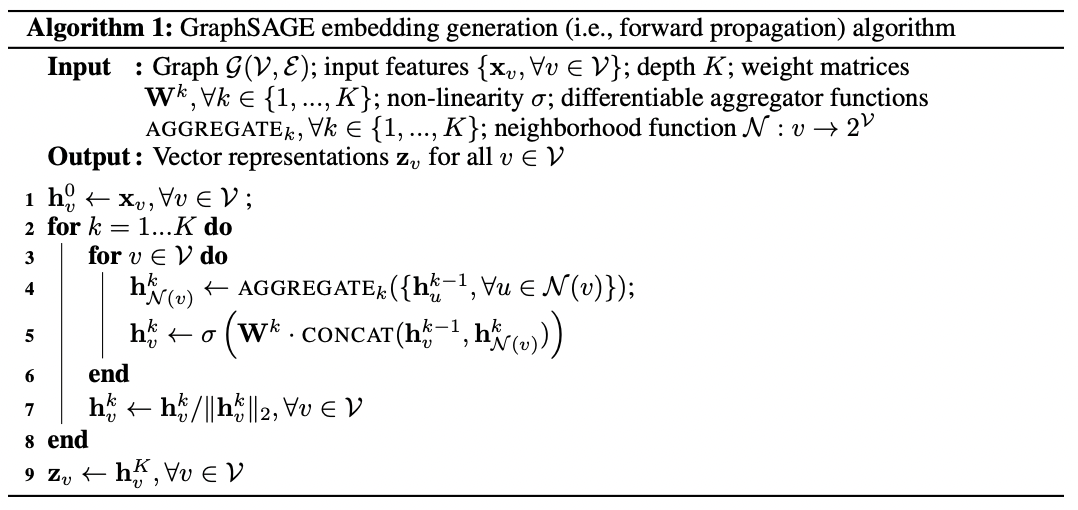
\includegraphics[width=0.5\textwidth]{GraphSAGE.png}
    \caption{\textsc{GraphSAGE} Algorithm \cite{Hamiltonetal.2017}}
    \label{fig:GraphSage}
\end{figure}
 
The aggregator functions the authors proposed to fit in line 4 and 5 of the algorithm above (\ref{fig:GraphSage}) would be one of three following:

1) \textbf{Mean Aggregator}: Nearly equivalent to the convolutional propagation rule used in a \textsc{GCN} \cite{Kipf&Welling2017}. But we can derive an inductive variant of the \textsc{GCN} \cite{Kipf&Welling2017} via the following formula:
\begin{align}
    \centering
    \mathbf{h}_v^k \leftarrow \sigma(\mathbf{W} \cdot MEAN( ({\mathbf{h}^{k-1}_v})  \cup  ({\mathbf{h}^{k-1}_u, \forall u \in N(v)})))
    \label{mean_agg}
\end{align} 

2) \textbf{Pooling Aggregator}: In this pooling approach, each neighbor’s vector is independently fed through a fully-connected neural network. Following this transformation, an elementwise max-pooling operation is applied to aggregate information across the neighbor set, which makes it symmetric and trainable. 
\begin{align}
    \centering
    AGGREGATE_k^{pool} =  max( { \sigma(\mathbf{W}_{pool} \mathbf{h}^k_{u_i} + \mathbf{b}), \forall u_i \in N(V)}
    \label{pool_agg}
\end{align} 
where max denotes the element-wise max operator and $\sigma$ is a nonlinear activation function. 

3) \textbf{LSTM Aggregator}:  Compared to the mean aggregator, LSTMs have the advantage of larger expressive capability. However, it is important to note that LSTMs are not inherently symmetric (i.e., they are not permutation invariant), since they process (and require) their inputs in a sequential manner. We chose to use this aggregator function for our implementation of the \textsc{GraphSage} model. \\

\textbf{GAT} : The \textsc{GATConv} is a foundational pillar of \textsc{Graph Attention Networks (GAT)} \cite{Velickovic2017}. it uses masked self-attention layers to solve the problem of convolution of the current image. The characteristics of neighbor nodes can be aggregated by stacking layers without the need for complex matrix operations nor knowing the entire graph structure upfront.

Computationally, it is highly efficient: the operation of the self-attentional layer can be parallelized across all edges, and the computation of output features can be parallelized across all nodes. No eigendecompositions or similar costly matrix operations are required. The time complexity of a single \textsc{GAT} attention head computing \textit{F'} features may be expressed as \textit{O}( |\textit{V}|\textit{FF'} + |\textit{E}|\textit{F'} ), where \textit{F} is the number of input features, and |\textit{V}| and |\textit{E}| are the numbers of nodes and edges in the graph, respectively. 

\begin{figure}[h]
    \centering
    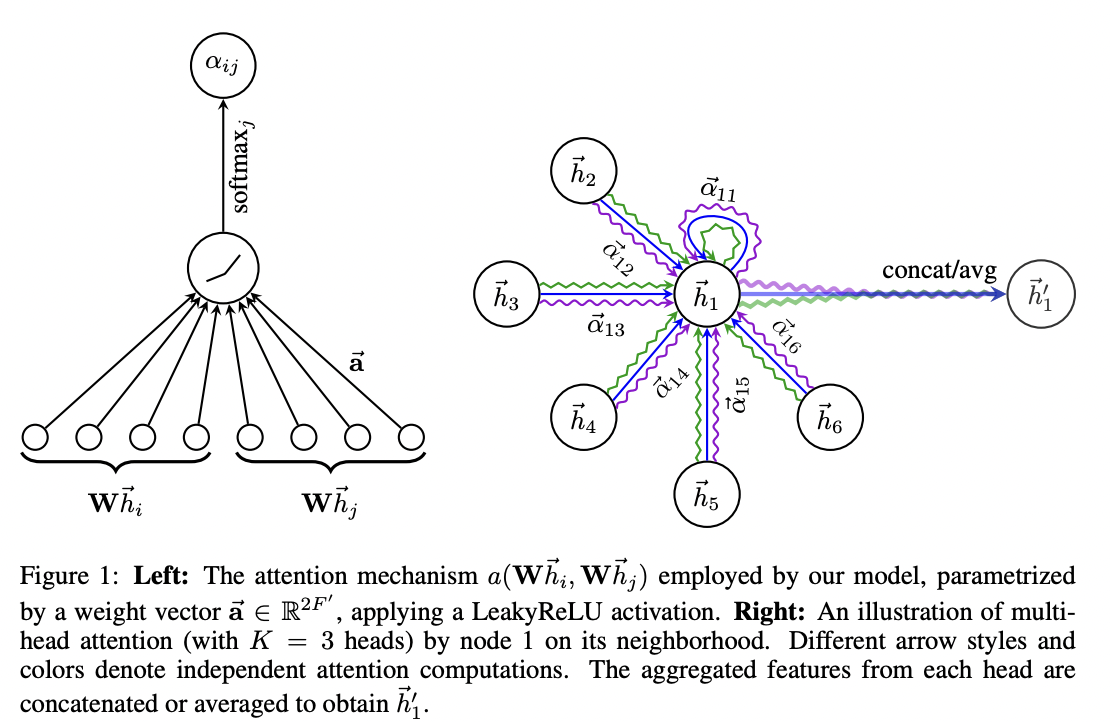
\includegraphics[width=0.5\textwidth]{GAT.png} 
    \caption{\textsc{GAT}Attention Mechanism \cite{Velickovic2017}}
    \label{fig:GAT}
\end{figure}

\textbf{Le\textsc{GCN}} : \textsc{Local Extrema Convolutional Layer (\textsc{LEConv})} \cite{LeConvPaper} is an extension of the simple \textsc{GCN} layer that finds the importance of nodes with respect to their neighbors using the difference operator. Internally, a \textsc{GCN} layer computes the importance $\phi = XW$ for each neighbour of a node and subsequently uses a weighted average over all neighbours. If a score of one node is very high, the scores of all its neighbours will be high too, because of the weighted averaging. 

On the other hand, \textsc{LEConv} uses the following rule to assign scores to neighbours of a node, which allows the network to select local extremas of neighbour scores and use a better aggregation over neighbourhood \cite{LeConvPaper}.
\begin{align} 
\phi_i = \sigma \left(x_i W_1 + \sum_{j \in \mathcal{N}_{(i)}} A_{ij} \left(x_i W_2 - x_j W_3\right) \right)
\end{align} 
where $W_1$, $W_2$, and $W_3$ are learnable parameters and $\in \mathcal{N}_{(i)}$ is the neighbourhood of node $i$.

\textbf{GATv2} : The model is developed by Brody et. al \cite{Brodyetal}, who saw there was room for improvement in the original \textsc{GAT} model \cite{Velickovic2017}. Since the linear layers (matrix product with the weight matrix and the dot product with attention coefficients) in the standard \textsc{GATConv} are applied right after each other, they can be collapsed into a single linear operation. As a result, the ranking of attended nodes is unconditioned on the query node. Said otherwise, the ranking (the argsort) of attention coefficients is shared (static) across all nodes in the graph. That's why the expressiveness power of simple \textsc{GATConv} layers is restricted. \textsc{GATv2Conv} fixes this problem by introducing adaptive attention mechanism, that allows the rankings of attention coefficients to differ from one node to another. Due to more flexible attention ratings, the \textsc{GATv2Conv}-based models have a greater expressiveness power and hence perform better.

The exact mechanism of this "fixing" is shown below. In \textsc{GATConv} layers, the dot product of attention coefficients and hidden representations are computed before a non-linearity (usually a Leaky ReLU). In \textsc{GATv2Conv}, the dot product is computed after a non-linearity is applied to a hidden representation.
\begin{align} \text{\textsc{GATConv}:} \quad e(\mathbf h_i, \mathbf h_j) = \sigma\left( \mathbf{a}^T \left[\mathbf W \mathbf h_i || \mathbf W \mathbf h_j \right] \right)
\end{align}
\begin{align} 
\text{\textsc{GATv2Conv}:} \quad e(\mathbf h_i, \mathbf h_j) = \mathbf{a}^T\sigma\left( \mathbf W\left[\mathbf h_i || \mathbf h_j \right] \right)
\end{align}

Each model contained a unique propagation step approach (e.g. \textsc{GraphSage} used only \textsc{SAGEConv} for each layer). Note, though, attention-based models had skip connections. The implementations can be found in our github repository \footnote{ \href{https://github.com/vincentwi/Graph_Neural_Networks_Amazon}{https://github.com/vincentwi/Graph\_Neural\_Networks\_Amazon}}. 

\subsection*{Dataset Description}
The ogbn-products dataset is an undirected and unweighted graph, representing an Amazon product co-purchasing network. Nodes represent products sold in Amazon, and edges between two products indicate that the products are purchased together.

The data was collected by crawling Amazon website and contains product metadata and review information about 548,552 different products (Books, music CDs, DVDs and VHS video tapes). The dataset was built by Bhatia et al. in 2016 \cite{Bhatia2016}.

Each product had a product description text: the text was one-hot encoded, and subsequently Principal Component Analysis (PCA) was applied to reduce the number of features to 100.

The product category is used as the target variable, and the excerpt below shows the some of the categories.
\begin{figure}[htp]
    \centering
    \includegraphics[width=4cm]{product}
    \caption{Product Categories in OGBN-Products}
    \label{fig:galaxy}
\end{figure}
\subsection*{Hyperparameters}
Since the dataset was quite large, we used a batch size of 256. We found that a bigger batch size usually resulted in a smoother convergence; however, we were not able to exceed 512 nodes per batch due to GPU RAM limitations. Also, after 20 epochs, the training set losses and accuracies began to plateau. Therefore, we trained all models for 20 epochs. Additionally, attention-based models (\textsc{GAT} and \textsc{GATv2} )\cite{Brodyetal}\cite{Velickovic2017} had 4 heads, but half as many hidden neurons in each layer as other 3 models. Finally, we used the ELU activation function with the dropout rate of 0.25. (When we used 0.5 as the dropout probability, the training went very slowly because the dropout was introducing too much noise.)

To set other hyperparameters, we ran each model several times to find reasonably good values. The table below presents a summary of finally used hyperparameters. \\ \\
\begin{tabularx}{0.48\textwidth} { 
  | >{\raggedright\arraybackslash}X 
  | >{\centering\arraybackslash}X 
  | >{\centering\arraybackslash}X
  | >{\centering\arraybackslash}X | }
 \hline
 \multicolumn{4}{|c|}{Hyperparameter Tuning}\\ \hline
 Model name & Layers & Hidden Units & Learning Rate\\ \hline
 \textsc{GraphSage} & 3 & 256 & 0.002\\ \hline
 \textsc{GCN}  & 3  & 256 & 0.003  \\ \hline
 Le\textsc{GCN}  & 3  & 256 & 0.003  \\ \hline
 \textsc{GAT} & 4  & 128 & 0.005  \\ \hline
 \textsc{GATv2} & 4  & 128 & 0.004  \\ \hline
\end{tabularx}

\subsection*{Mini-Batch Strategy}
To construct our mini batches for training, we extracted random subgraphs from our training graph. For a given node, we randomly sampled 20 one-hop neighbours, 15 two-hop neighbours and 10 three-hop neighbours, shuffling the order of nodes in each epoch.

However, when we evaluated accuracy, we used all available neighbours not only in the validation and test sets, but also in the training set. In our opinion, this gives a more accurate reflection of the training set performance compared to model evaluation on the subgraphs with limited number of neighbours.

\section*{Results and Discussion}

\subsection*{Exploratory Data Analysis} 
Overall, the ogbn-products dataset contains 2,449,029 nodes and 123,718,280 edges. We have split them into three categories based on the above-mentioned method to have 196,615 nodes for training, 39,323 nodes for model tuning and validation, and 2,213,091.

Out of the 47 target categories, the most represented classes were Books (668,950 nodes), CDs and Vinyl (172,199 nodes), Toys and Games (158,771 nodes) and Sports and Outdoors (151,061 nodes). The most underrepresented classes were Purchase Circles (29 nodes), Furniture and Decor (9 nodes), and Digital Music (9 nodes).

More than 84\% of the nodes had a degree of 1, around 13\% had a degree of 2, and only 3\% had a degree of 3 or above.

\subsection*{Comparison of Models}

For comparing the performance of the models, we used accuracy as a metric. Below, the performances on the training, validation and test sets are given for each model.\\ \\
\begin{tabularx}{0.48\textwidth} { 
  | >{\raggedright\arraybackslash}X 
  | >{\centering\arraybackslash}X 
  | >{\centering\arraybackslash}X
  | >{\centering\arraybackslash}X | }
 \hline
 \multicolumn{4}{|c|c|}{Model Accuracies (\%)}\\ \hline
 Model name & Train & Validation & Test\\ \hline
 \textsc{GraphSage} & 90.09 & 88.24 & 78.45\\ \hline
 \textsc{GCN}  & 89.76  & 88.46 & 76.64 \\ \hline
 Le\textsc{GCN}  & 92.66  & 90.26 & 82.59 \\ \hline
 \textsc{GAT} & 91.10  & 89.42 & 79.19 \\ \hline
 \textsc{GATv2} & 93.38  & 91.57 & 84.27 \\ \hline
\end{tabularx} \\ \\

Our results show that training set and validation set accuracies of different models do not differ significantly. However, their generalization power displays a greater degree of variety. The best performing models were Local Extremum GNN \cite{LeConvPaper} and Dynamic \textsc{GAT}\cite{Brodyetal}.  The former achieved 92.7\% accuracy on the training set and 82.6\% on the test set. The latter performed marginally better, with 93.4\% training accuracy and 84.3\% test accuracy. Meanwhile, \textsc{GraphSage} \cite{Hamiltonetal.2017} achieved a reasonably high accuracy (90.1\% on the training set and 78.5\% on the test set), despite being a relatively simple model.

If we compare the performances of Local Extremum GNN \cite{LeConvPaper} and Dynamic Graph Attention Networks \cite{Brodyetal} with their initially proposed versions (Graph Convolutional Networks and static GATs) \cite{Kipf&Welling2017} \cite{Velickovic2017}, we can see that adaptive aggregation in \textsc{LEConv} layers and adaptive attention mechanism in \textsc{GATv2}\cite{Brodyetal} layers do offer a performance advantage: for \textsc{GCN}s, the test set accuracy boost was almost 6\%, while it was slightly over 5\% for GATs.

We can infer that the reason \textsc{GAT}models \cite{Velickovic2017} perform better than a baseline method like \textsc{GCN} \cite{Kipf&Welling2017} is due to the fact it  allows for (implicitly) assigning \textit{different importances} to nodes of a same neighborhood. However, this complexity of GATs is on par with \textsc{GCN}s, since as we said previously, they don't require complex matrix calculations. 

Finally, the generalization gap for all models was quite significant. The difference between the training set and test set accuracies was between 9\% and 13\% for all models. The tightest difference was recorded by the dynamic \textsc{GAT}model \cite{Brodyetal} (9.1\%) and the widest by the \textsc{GCN} model \cite{Kipf&Welling2017} (13.1\%). Validation accuracies were usually within 1-2\% from the respective training set accuracies. To assess the impact of the chosen split on the models' generalization power, we applied the same split (8\% training, 2\% validation and 90\% test) using stratified sampling. The accuracy was 91.6\%, 90.1\%, and 88.9\% on the training, validation, and test sets, respectively. This training-test accuracy difference of 1.7\% implies that the sales-ranking-based split poses a more challenging task than a random stratified split. However, we believe that using this split offers a realistic comparison among models and more closely reflects the real-life generalization power of the above graph neural networks.

\section*{Conclusion}
Over the past few years, graph neural networks have become powerful and practical tools for machine learning tasks in graph domains. This progress owes to advances in expressive power, model flexibility, and training algorithms. In this paper, we replicate several key graph neural networks. For GNN models, we categorize its variants by its propagation modules: 1) Spectral, 2) Spacial, 3) Attention-based Spacial.

Our results show that a model using \textsc{GATv2Conv} layers \cite{Brodyetal} achieved the highest accuracy, while the one having simple \textsc{GCN} models \cite{Kipf&Welling2017} had the worst performance. Also, attention-based models had a better generalization power, as illustrated by the training accuracy-test accuracy gap, while \textsc{GCN}-layer models had a wider gap between the performances on the two sets.

Also, we discovered that a sales-ranking-based split is a more challenging problem than a random stratified sampling, where models can achieve a very high results (88\% test accuracy).

There is still a lot of work to be done in robustness, interpretability, pretraining and complex structure modeling, but we are thankful to have had the opportunity to explore these 5 graph neural network models. 

\medskip


\printbibliography

\end{document}


                                                                                                                                                                                                                                                                                                                                                                                                                                                                  